\documentclass[sigplan,screen]{acmart}\settopmatter{printfolios=true,printccs=false,printacmref=false}
%\documentclass[acmsmall,review,anonymous]{acmart}\settopmatter{printfolios=true,printccs=false,printacmref=false}

\usepackage[utf8]{inputenc}
\usepackage[T1]{fontenc}

\usepackage{adjustbox}
\usepackage{booktabs}
\usepackage{listings}
\usepackage{multicol}
\usepackage[autolanguage]{numprint}
\usepackage{proof}
\usepackage{softdev}
\usepackage{stmaryrd}
\usepackage{setspace}
\usepackage{subcaption}
\usepackage{wrapfig}
\usepackage{xspace}
\usepackage{menukeys}
\usepackage[normalem]{ulem}

\usepackage[ruled]{algorithm2e} % For algorithms
\renewcommand{\algorithmcfname}{ALGORITHM}
\SetAlFnt{\small}
\SetAlCapFnt{\small}
\SetAlCapNameFnt{\small}
\SetAlCapHSkip{0pt}
\IncMargin{-\parindent}

%\acmJournal{SLE}
%\acmVolume{1}
%\acmNumber{CONF} % CONF = POPL or ICFP or OOPSLA
%\acmArticle{1}
%\acmYear{2019}
%\acmMonth{1}
%\acmDOI{} % \acmDOI{10.1145/nnnnnnn.nnnnnnn}
\acmConference[SLE'19]{Software Language Engineering}{October 2019}{Athens, Greece}
\startPage{1}

\lstset{
    basicstyle=\ttfamily\scriptsize,
    xleftmargin=0pt,
    numbersep=.8em,
    numberstyle=\scriptsize\tt\color{gray},
    captionpos=b,
    escapeinside={{<!}{!>}},
}

% from https://tex.stackexchange.com/questions/264361/skipping-line-numbers-in-lstlisting#264373
\let\origthelstnumber\thelstnumber
\makeatletter
\newcommand*\Suppressnumber{%
  \lst@AddToHook{OnNewLine}{%
    \let\thelstnumber\relax%
     \advance\c@lstnumber-\@ne\relax%
    }%
}

\newcommand*\Reactivatenumber[1]{%
  \setcounter{lstnumber}{\numexpr#1-1\relax}
  \lst@AddToHook{OnNewLine}{%
   \let\thelstnumber\origthelstnumber%
   \refstepcounter{lstnumber}
  }%
}

\setcopyright{none}

\bibliographystyle{ACM-Reference-Format}
\citestyle{acmauthoryear}

% DOI
%\acmDOI{0000001.0000001}

% Paper history
%\received{February 2007}

\newcommand{\inputtree}[0]{\emph{CST}\xspace}
\newcommand{\eco}[0]{\emph{Eco}\xspace}
\newcommand{\ald}[0]{\emph{ALD}\xspace}
\newcommand{\qtt}[1]{`\texttt{#1}'\xspace}

\newcommand{\hotkeynewlbox}[0]{\keys{Ctrl+L}\xspace}
\newcommand{\hotkeyleavelbox}[0]{\keys{Ctrl+Shift+L}\xspace}

\newcommand{\validalljavalua}{99.4\%\xspace}
\newcommand{\validalljavaphp}{94.6\%\xspace}
\newcommand{\validalljavasqlite}{99.7\%\xspace}
\newcommand{\validallluajava}{97.9\%\xspace}
\newcommand{\validallluaphp}{95.9\%\xspace}
\newcommand{\validallluasqlite}{97.6\%\xspace}
\newcommand{\validallphpjava}{99.2\%\xspace}
\newcommand{\validallphplua}{99.2\%\xspace}
\newcommand{\validallphpsqlite}{100.0\%\xspace}
\newcommand{\validallsqlitejava}{97.9\%\xspace}
\newcommand{\validallsqlitelua}{95.2\%\xspace}
\newcommand{\validallsqlitephp}{94.3\%\xspace}
\newcommand{\validalloverall}{97.6\%\xspace}
\newcommand{\validhistjavalua}{67.4\%\xspace}
\newcommand{\validhistjavaphp}{90.7\%\xspace}
\newcommand{\validhistjavasqlite}{99.5\%\xspace}
\newcommand{\validhistluajava}{97.5\%\xspace}
\newcommand{\validhistluaphp}{86.2\%\xspace}
\newcommand{\validhistluasqlite}{90.0\%\xspace}
\newcommand{\validhistphpjava}{95.9\%\xspace}
\newcommand{\validhistphplua}{53.1\%\xspace}
\newcommand{\validhistphpsqlite}{100.0\%\xspace}
\newcommand{\validhistsqlitejava}{96.8\%\xspace}
\newcommand{\validhistsqlitelua}{99.0\%\xspace}
\newcommand{\validhistsqlitephp}{96.8\%\xspace}
\newcommand{\validhistoverall}{89.4\%\xspace}
\newcommand{\validstackjavalua}{97.6\%\xspace}
\newcommand{\validstackjavaphp}{94.5\%\xspace}
\newcommand{\validstackjavasqlite}{99.5\%\xspace}
\newcommand{\validstackluajava}{96.2\%\xspace}
\newcommand{\validstackluaphp}{94.3\%\xspace}
\newcommand{\validstackluasqlite}{69.4\%\xspace}
\newcommand{\validstackphpjava}{99.2\%\xspace}
\newcommand{\validstackphplua}{98.1\%\xspace}
\newcommand{\validstackphpsqlite}{100.0\%\xspace}
\newcommand{\validstacksqlitejava}{97.5\%\xspace}
\newcommand{\validstacksqlitelua}{95.2\%\xspace}
\newcommand{\validstacksqlitephp}{94.0\%\xspace}
\newcommand{\validstackoverall}{94.6\%\xspace}
\newcommand{\validlinejavalua}{97.5\%\xspace}
\newcommand{\validlinejavaphp}{79.3\%\xspace}
\newcommand{\validlinejavasqlite}{99.2\%\xspace}
\newcommand{\validlineluajava}{98.2\%\xspace}
\newcommand{\validlineluaphp}{96.2\%\xspace}
\newcommand{\validlineluasqlite}{96.5\%\xspace}
\newcommand{\validlinephpjava}{99.2\%\xspace}
\newcommand{\validlinephplua}{98.2\%\xspace}
\newcommand{\validlinephpsqlite}{99.7\%\xspace}
\newcommand{\validlinesqlitejava}{97.9\%\xspace}
\newcommand{\validlinesqlitelua}{99.3\%\xspace}
\newcommand{\validlinesqlitephp}{96.1\%\xspace}
\newcommand{\validlineoverall}{96.4\%\xspace}
\newcommand{\breakdownallvalid}{72.2\%\xspace}
\newcommand{\breakdownallinvalid}{1.8\%\xspace}
\newcommand{\breakdownallnovalid}{22.6\%\xspace}
\newcommand{\breakdownallnoerror}{0.7\%\xspace}
\newcommand{\breakdownallnomulti}{2.8\%\xspace}
\newcommand{\breakdownhistvalid}{63.7\%\xspace}
\newcommand{\breakdownhistinvalid}{0.6\%\xspace}
\newcommand{\breakdownhistnovalid}{22.4\%\xspace}
\newcommand{\breakdownhistnoerror}{10.0\%\xspace}
\newcommand{\breakdownhistnomulti}{3.2\%\xspace}
\newcommand{\breakdownstackvalid}{69.4\%\xspace}
\newcommand{\breakdownstackinvalid}{1.8\%\xspace}
\newcommand{\breakdownstacknovalid}{22.5\%\xspace}
\newcommand{\breakdownstacknoerror}{3.6\%\xspace}
\newcommand{\breakdownstacknomulti}{2.8\%\xspace}
\newcommand{\breakdownlinevalid}{70.7\%\xspace}
\newcommand{\breakdownlineinvalid}{1.1\%\xspace}
\newcommand{\breakdownlinenovalid}{22.5\%\xspace}
\newcommand{\breakdownlinenoerror}{2.5\%\xspace}
\newcommand{\breakdownlinenomulti}{3.2\%\xspace}


\lstnewenvironment{lstdefault}[1][]
  {
    \lstset{
        numbers=left,
        language=Python,
        keywordstyle=\color{red!70!black},
        commentstyle=\itshape\color{gray!90!black},
        stringstyle=\color{green!60!black},
        basicstyle=\linespread{0.9}\footnotesize\ttfamily,
        numberstyle=\tiny,
        keepspaces=true,
        breaklines=true,
        captionpos=b,
        abovecaptionskip=0.8em,
        columns=fullflexible,
        xleftmargin=10pt,
        aboveskip=1em,
        belowskip=0em,
        showstringspaces=false,
        literate={\$}{{\$}}1,
        escapeinside={{<!}{!>}},
        #1
    }
}{}

\lstdefinelanguage{EcoGrammar}
{
    alsoletter={:,\:=,|},
    morekeywords={:, =, | },
    keywordstyle=\color{red!70!black},
    morestring=[b]",
    stringstyle=\color{green!60!black},
    commentstyle=\itshape\color{gray!90!black},
    comment=[l]{//},
    morecomment=[s]{/*}{*/},
}

\lstnewenvironment{lsteco}[1][]
  {
    \lstset{
        language=EcoGrammar,
        basicstyle=\footnotesize\ttfamily,
        numberstyle=\tiny,
        xleftmargin=10pt,
        showstringspaces=false,
        #1
    }
}{}

% Document starts
\begin{document}
% Title portion. Note the short title for running heads
\title{Automatic Language boxes}

\author{Lukas Diekmann}
\affiliation{%
  \department{Software Development Team}
  \institution{King's College London}
  \country{United Kingdom}}
\author{Laurence Tratt}
\orcid{0000-0002-5258-3805}
\affiliation{%
  \department{Software Development Team}
  \institution{King's College London}
  \country{United Kingdom}
}
\thanks{Authors' URLs: %
    L.~Diekmann~\url{http://lukasdiekmann.com/},
    L.~Tratt~\url{http://tratt.net/laurie/}.
}


\begin{abstract}
Since composed grammars are often ambiguous, grammar composition requires a
mechanism for dealing with ambiguity: either ruling it out entirely through the use of
delimiters, or by selecting the desired parse tree from the parse forest.  In
this paper we show that \emph{language boxes} -- a delimiter-based
algorithm atop incremental parsing -- can be extended in a way that creates
a new point in the design space between these two extremes. In essence, we
retain the use of delimiters, but
introduce an algorithm which can automatically insert, remove, or resize
language boxes -- leading to what we call \emph{automatic language
boxes}. The very nature of the problem means that automatic language boxes
cannot always match a user's intention: rather, we present a simple
algorithm that does the right thing in most cases, while rarely surprising the
user when it cannot.
\end{abstract}

\keywords{Parsing, language composition, programming languages}

\maketitle

\section{Introduction}

\begin{figure*}
    \vspace{1em}
    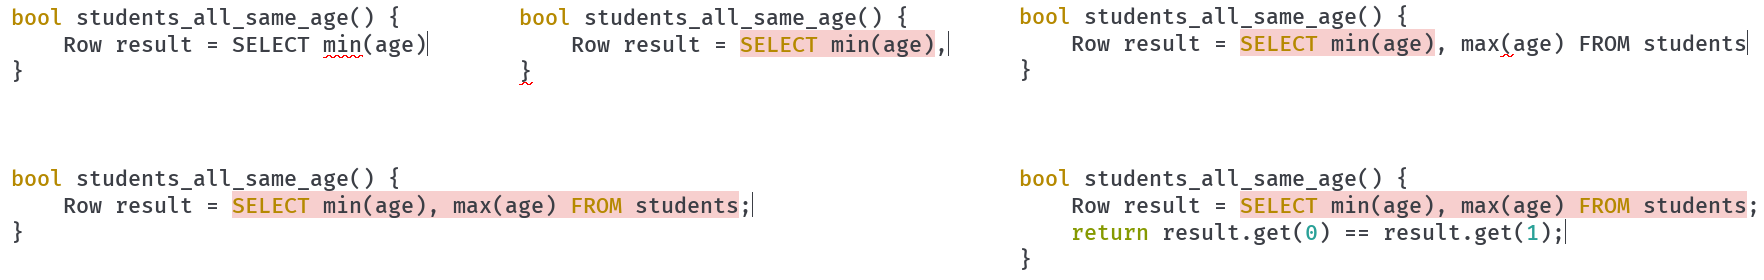
\includegraphics[width=1.00\textwidth]{images/mainexample_java_sql}
    \begin{picture}(0,0)
        \put(-249,103){\textcolor{black}{\textbf{(a)}}}
        \put(-103,103){\textcolor{black}{\textbf{(b)}}}
        \put(  40,103){\textcolor{black}{\textbf{(c)}}}
        \put(-249,51){\textcolor{black}{\textbf{(d)}}}
        \put(  40,51){\textcolor{black}{\textbf{(e)}}}
    \end{picture}
    \vspace{-2.2em}
    \caption{An example of automatic language boxes in action (with elided screenshots from our
      extension to the Eco editor). Here, the user is entering text in a
      composition of Java and SQL, where SQL statements can be used wherever
      Java expressions are valid. As the user types, language boxes (with a
      pink background) are automatically inserted, removed, or resized.
      \textbf{(a)} After typing the skeleton of a Java function, the user begins
      typing an SQL statement as the right-hand side expression of a Java
      assignment. The most fundamental part of the
      algorithm is to try inserting language boxes when a syntax error in the
      outer language occurs (as can be seen at the \texttt{min} function) but
      not if it then leads to a syntax error immediately after the inserted
      language box. It is thus too early to insert an automatic language box
      around the SQL as it would cause a syntax error in the first non-whitespace token
      afterwards (`\texttt{,}'). \textbf{(b)} After typing `\texttt{,}' an SQL
      language box is automatically inserted since the next non-whitespace Java token
      (`\texttt{,}') is now syntactically valid. \textbf{(c)} The user continues
      typing a (now incomplete) SQL statement. This causes syntax errors in the
      outer language which cannot yet be resolved by inserting, removing, or
      resizing any language boxes.  \textbf{(d)} After typing `\texttt{;}', the
      automatic language box algorithm resizes the existing language box to
      encompass the entire SQL statement, making the program syntactically
      complete. \textbf{(e)} Further syntactically correct Java input does not
      cause the language box to be altered.
}
\label{intro_example}
\end{figure*}

Language composition -- the ability to build larger languages out of multiple
small languages -- offers an enticing solution to problems such as the
development of domain-specific languages or the migration of legacy software.
Unfortunately, writing and editing composed programs is often cumbersome.
The basic problem is that grammar
composition -- which underpins language composition -- can cause
two provably unambiguous grammars to become ambiguous when composed,
and determining whether a grammar is unambiguous or not is
undecidable~\cite{cantor62ambiguity}. There are two fundamental approaches
of coping with ambiguity: either ruling it out through the use of
delimiters (either via explicit bracketing or syntax-directed
editing); or using a generalised parsing algorithm that can create a parse
forest, capturing all ambiguities
(e.g.~\cite{visser97scannerless}). Each has different trade-offs: delimiters
are visually intrusive and/or awkward to work with; and one can never know if all possible
ambiguous parses have been covered by disambiguation operators.

An alternative to traditional delimiter-based approaches are \emph{language boxes} which aim to
combine the advantages of explicit bracketing and syntax-based
editing~\cite{diekmann14eco}. In essence, an editor
which supports language boxes needs to support an incremental parsing algorithm
(we assume that of~\citet{wagner98practicalalgorithms}), which provides an
online editing experience: unlike traditional editors, users are not editing
a contiguous block of text in memory, but instead
indirectly edit a parse tree, which is continuously updated as they type.
Language boxes are then simply nodes in a parse
tree that represent a different language: the language box is surrounded by
explicit, but invisible, delimiters. Unlike explicit bracketing approaches,
there are no visually intrusive delimiters; unlike traditional
syntax-based editors, the program can be syntactically incorrect in arbitrary
ways and places during editing. However, language boxes lack the most appealing aspect of
ambiguous parsing: users must explicitly, and tediously, state when they want
to insert or remove language boxes.

The fundamental research question underlying this paper is whether it is
possible to reduce the need for the users to explicitly insert and remove language
boxes. For example, in a composition of Java and SQL (where SQL is allowed
wherever a Java expression is valid), can such a system automatically insert an
SQL language box around the SQL in \texttt{for (String n: SELECT name FROM table) \{ ...
\}}? It is important to acknowledge from the outset that a perfect solution
is impossible, since there will always be some cases where there are multiple
ways of splitting the same input across different language boxes. Realistic
solutions must also take into account other considerations: it should not
require significant extra work for the authors of composed languages; performance must
not be unduly impacted; and users should be able to broadly predict if, and
why, language boxes are inserted or removed.

The solution we present to this problem are \emph{automatic language boxes}. In
essence, we present an algorithm which can automatically insert, remove, or resize language
boxes in many useful cases. The algorithm is, in essence, comprised of several
stages: determining what user inputs should trigger it; finding candidate language
boxes to insert, remove, or resize; filtering out those which would make the
overall program worse; and then applying them. One of the main challenges with
automatic language boxes is to determine what portion of the program to search
for possible language boxes: we present several heuristics for this case
(including the ability to take the user's previous input into consideration)
which, when combined, lead to an effective heuristic for many cases. Figure
\ref{intro_example} shows a simple example and walks readers through the high-level
parts of the algorithm and accompanying heuristics.

We implemented automatic language boxes as an extension to the Eco
editor~\cite{diekmann14eco}. In order to validate automatic language boxes, we
created several language compositions involving large, real-world languages,
and composed programs in those compositions by extracting fragments from real-world programs.
In other words, our experiment is equivalent to opening a file
in one language, moving the cursor to a given position, deleting a fixed amount
of text, and then inserting text one character at a time from another language.
Our experiments show that in \validalloverall of cases, automatic language boxes achieve an
acceptable result by which we mean they either: inserted a single valid
language box (\breakdownallvalid); did not insert a language box because the
inserted fragment was valid in both languages (\breakdownallnovalid); or an ambiguity
was found and there were multiple different ways of inserting language boxes
(\breakdownallnomulti). As this suggests, the number of cases where automatic
language boxes perform poorly is small and is split into two categories: a
language box was inserted, but syntax errors remain because not all of the
input was put into the language box (\breakdownallinvalid); or a language box wasn't
inserted when we would have expected it to be (\breakdownallnoerror). Our fully
repeatable experiment can be found at \emph{redacted for double blind review}
and our extensions to the Eco editor can be found at \emph{redacted for double
blind review}.


\section{Background}
\label{sec_background}

In this section, we briefly survey existing approaches to editing composed
programs, before giving a brief overview of incremental parsing, sufficient for
this paper's purposes.


\subsection{Delimiter-based approaches}

The traditional approach to language composition is to use delimiters
to make clear when the user has switched from one sub-language to another. The
most obvious way of achieving this is to use explicit brackets to make clear a
switch from an outer to an inner language (e.g.~\texttt{for (String e: <<SELECT name
FROM table>>) \{ ... \}}), though this is visually intrusive, and prevents the
brackets being used within the sub-language (e.g.~in this case, the sub language
cannot use `\texttt{>>}' as a bit-wise operator).

Naive approaches inherit a severe restriction from traditional parsing, which
separates lexing (i.e.~the splitting of the user's input into tokens) from
parsing (i.e.~the structuring of tokens into a parse tree): all the languages
must share the same lexing rules. This restriction can be somewhat eased if the
lexer recognises the explicit brackets and extracts text between them wholesale
for separate lexing and parsing (see e.g.~\cite[p.~13-14]{tratt08domainspecific}),
though it is then hard for the lexer to accurately keep track of nested
brackets (e.g.~should brackets in comments be counted or not? and how does
one know what format comments in the inner language(s) are in?).  A
more sophisticated approach is for the lexer and parser to interact (see
e.g.~\cite{wyk07context}), such that the parse causes a switch in lexing rules
when input shifts to an inner language.
This has the advantage that brackets do not always need to be quite as visually
intrusive (e.g.~one can use a difference in keywords to identify a switch from
one language to another), though in the general case explicit brackets must still be
used to resolve ambiguities.


\subsection{Scannerless parsing}
\label{sec:scannerless}

Generalised parsing can parse any Context-Free Grammar (CFG), even those that
are ambiguous. Scannerless parsing~\cite{visser97scannerless} extends this such
that lexing and parsing are specified together. This removes the need for
explicit brackets entirely, but does so at the expense of causing many more
ambiguities (since traditional lexers implicitly resolve many ambiguities, such
as between identifiers and keywords, before parsing).
This is challenging because ambiguity is, in general,
undecidable~\cite{cantor62ambiguity} and even the best ambiguity heuristics fail
to find all possible sources of ambiguity~\cite{vasudevan13detecting}. Thus,
no matter how many static disambiguation operators one uses, in general one
cannot be sure if all possible points of ambiguity have been covered.
Furthermore, our current disambiguation operators can cause scannerless
parsers to become context-sensitive~\cite{eijck__lets_accept_rejects}, the
consequences of which remain unclear.


\subsection{Syntax directed editing}

Traditional syntax directed editing avoids parsing text entirely. In essence,
users edit an AST directly, with incomplete parts of a program being
represented by holes. This avoids the need for explicit delimiters, and
sidesteps issues of ambiguity completely. However, such systems are awkward to
use~\cite[p.~2]{khwaja93syntax}, for example only allowing whole nodes in the AST to be selected at a time,
and quickly fell out of fashion. The modern syntax directed editor
MPS~\cite{pech13mps} alleviates some, though not all, of these problems.
However, it requires significant expertise on the part of the composition
author to make editing a pleasant experience, as the AST structure places
constraints on many editing operations.


\subsection{Incremental parsing}

Parsing is traditionally a batch process: an entire file is fed through a parser
and a parse tree created from it. Incremental parsing, in contrast,
continually parses text and updates a parse tree as the user types.
In this paper we make use of the incremental lexing and
LR incremental parsing algorithms of~\citet{wagner98practicalalgorithms},
taking into account the several fixes found in~\cite{diekmann18editing}.
In this subsection we provide a brief overview of this algorithm sufficient
to understand the rest of this paper.

The incremental lexer and parse both operate on the parse tree. Parse tree nodes
are either \emph{nonterminals} (representing rules in the grammar) or
\emph{tokens} (representing terminal symbols). Nonterminal nodes have an
immutable type (e.g.~`expr') but the quantity and types of their children can change.
Tokens have a mutable type (e.g.~`int')
and a mutable value (e.g.~`3') but cannot have children at all.

After input from the user is received, the incremental lexer is run first.
Using lookahead information, it works out the affected area of the change,
updates or creates tokens as necessary, and marks the path from each updated or
created token to the root as changed. The incremental parser then runs,
reparsing all subtrees with changes in them, and creating or removing
nonterminals as needed. Syntax errors mean that a fully correct parse tree
cannot be created, in which case some tokens will be attached, in a sense
temporarily, to the nearest parent, until a correct parse can be created.


\subsection{Language boxes}

\begin{figure}[t]
\begin{center}
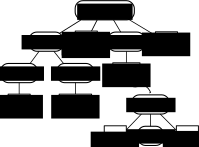
\includegraphics[width=0.35\textwidth]{images/lbox_parsetree}
\caption{An elided example of a parse tree in an incremental parser with
  language boxes: nonterminals have a type and zero or more children; terminals
  have a type (top) and a value (bottom). The composition in question is,
  again, (outer) Java and (inner) SQL. Here, the outer Java code is an
  assignment (`\texttt{type name = ...;}'). The right-hand side of the
  assignment is an SQL language box (the node with type \texttt{<sql>}): from the
  perspective of the outer Java code, the SQL node is a terminal (and hence its
  value is irrelevant). In reality, the SQL node has a complete SQL parse tree
  underneath it: the special Root, BOS (Beginning Of String), and EOS (End Of
  String) nodes that every incremental parse tree contains, as well as the actual
  SQL contents (elided to `...' in this example). }
\label{fig:lboxtree}
\end{center}
\end{figure}

Language boxes allow users users to embed one language inside another in the
context of an incremental parser. From the perspective of an outer language, a
language box is simply a terminal i.e.~a node with a type but no content. Since
parsers only care about the type of a terminal, this is a natural fit. In
reality, language boxes do have content, though it is not visible to the outer
language: they contain a separate parse tree for the inner language within
them.

This simple definition belies its power. Consider a composition of Java and
SQL, where SQL expressions can be used wherever a Java expression is
syntactically valid. Java's grammar must have a reference from Java's
expression rule to a special symbol type `language box' (conventionally
represented between angle brackets to visually separate it from rules and
tokens). At run-time, if the Java parse tree has an SQL language box at the
correct point, then Java considers the tree to be syntactically correct. The
SQL language box will have its own SQL parse tree inside which may or may not
be syntactically correct. An elided example of such a tree-of-trees can be seen
in Figure~\ref{fig:lboxtree}.

Philosophically, language boxes thus form delimiters of sorts, albeit invisible
ones, between languages: from a syntactic perspective, outer languages are
ignorant of the contents of inner languages and vice versa. Thus we get much of
the power of syntax-directed editing without the accompanying difficulty of
editing ASTs. At all points, all languages can be manipulated as normal text
using the incremental parsers.


\section{Beyond manual language boxes}

\label{the problem}
The chief weakness of language boxes is that they must be inserted
manually by the user --- this involves pressing a special key combination,
selecting the desired inner language from a list, typing the content, and (in
general) pressing a second special key combination to complete the language box.
When language boxes are used infrequently, this is merely irritating,
but when language boxes are used frequently, it is a significant usability
issue, impeding the user's flow. Eco, an editor which supports language boxes~\cite{diekmann14eco},
slightly eases this problem by using information from the incremental parser to
show only those languages valid at the point of the cursor,
though this is a mild palliative at best. A superior solution would be
to automatically insert, remove, and resize language boxes whenever possible.

In an ideal world, we would be able to insert language boxes exactly, and only,
when they are wanted by the user. However, this is impossible in the
general case because language composition is really grammar composition
in disguise, and thus subject to the same ambiguity problems as generalised
parsing (see Section~\ref{sec:scannerless}). Even if we were to require the
language composition author to provide a static disambiguation specification,
we cannot guarantee that it will cover all the ambiguous
possibilities. Annoying as this may be, it is a hard constraint that we cannot
change. On top of this, we also assert that a realistic solution to automatic
language boxes should satisfy several softer considerations.

First, a solution which requires language composition authors (i.e.~the people
who actually compose grammars, create code generators etc.) to provide additional
hints or commands to aid automatic language box insertion is less likely
to be used widely and/or correctly. The meta-system underlying a language
composition system is often complex, and expecting language composition authors
to be expert in every part of it (as well as the domain they are composing
languages for!) is unrealistic. For example, it can be difficult to know whether
a non-LR grammar is ambiguous or not~\cite{vasudevan13detecting} and whether
one has disambiguated it in the expected way: grammar
composition often magnifies such concerns.

Second, a solution which seriously degrades performance would be unacceptable.
For example, one simple way of finding which language boxes to insert would
be to reparse the complete file on every keypress, which would be noticeably slow for large
files. Ideally, the theoretical performance guarantees
of~\citet{wagner98practicalalgorithms} would be maintained as well as good
practical performance\footnote{Interestingly, the original implementation of
this incremental parsing algorithm had to be triggered by the user (e.g.~when
a file was saved). Modern machines are fast enough that even a naive
implementation can run comfortably on every keypress in nearly all reasonable
cases.}.

Third, a solution which inserts language boxes unpredictably would be unlikely
to find favour with users. Clearly, given the hard constraint described at the
start of this subsection, users cannot expect perfect language box insertion
all of the time. However, a reasonable minimum expectation is that it should be
entirely predictable as to when automatic language boxes are potentially
inserted, removed, or
resized; and, ideally, largely predictable as to what the effects of such
actions are. Furthermore, false negatives (i.e.~when the system inserts, removes,
or resizes language boxes incorrectly) are likely to be particularly harshly
received by users and must be reduced to the minimum possible, given the hard
constraint above.


\section{Automatic language boxes}

In this section, we present the automatic language boxes algorithm. To ease its
description, we start by considering the problem of language box
insertion, before then adding additional functionality (e.g.~removal and
resizing). We later validate the usefulness of automatic language boxes in
Section~\ref{sec:evaluation}.


\subsection{The consideration heuristic}

The first challenge with automatic language boxes is to decide upon a sensible
heuristic for considering if/when to insert a language box -- what we call the
\emph{consideration heuristic}. If the consideration heuristic triggers too
frequently, it will lead to too many unwanted language boxes being inserted,
each of which must then be manually removed by the user.
Conversely, if it triggers infrequently, it will not be a useful aid to the user.

We use two related observations as the guides to our consideration heuristic.
First, by definition, language composition always consists of an outer language
and one or more inner languages\footnote{Note that these terms are relative:
when we create a language box and move into it, the previously-inner language
now becomes the outer language.}. It is thus a reasonable expectation that most
text typed in the outer language is intended to be in the outer language.
Second, the clearest indication that recently typed text in the outer language
might have been intended for an inner language is that it leads to a syntax error
in the outer language.

\begin{figure}[tb]
    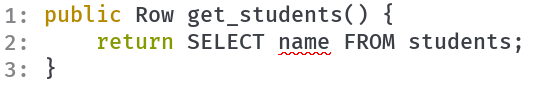
\includegraphics[width=.45\textwidth]{images/composition_error1.png}
    \caption{An example of a syntax error in a Java and SQL composition. In
      this example, we have turned off automatic language box insertion to
      emphasise the fact that syntax errors often occur in the middle of the
      language box we would like to insert.}
\label{fig:consideration}
\end{figure}

Our consideration heuristic therefore triggers at the point of each new syntax error.
This is an entirely predictable heuristic from a user perspective, though it
does have two consequences: the point of a syntax error is not always at the
beginning or end of the text that a user expects to be put in a language box
(see Figure~\ref{fig:consideration}); and this heuristic clearly works better
for languages whose syntaxes don't overlap a great deal. Happily, we can rely
on the fact that the incremental parser isolates syntax errors after they
occur~\cite[p.~93]{wagner98practicalalgorithms}, so that there is no
possibility of old syntax errors being considered a second time.


\subsection{The candidates heuristic}

Once the consideration heuristic has triggered, we then have to search for
plausible language boxes to insert -- we call this the \emph{candidates heuristic}. A candidates heuristic
can produce zero or more candidate language boxes at any given point; those
candidate language boxes may cover different spans and/or be of different
language types. Note that candidates heuristics merely need to suggest language
boxes which consume existing content: the subsequent phase in the algorithm
then determines if actually inserting such language boxes makes sense in the
wider context of the program (see Section~\ref{sec:filtering}).

Before we can define candidates heuristics, we first need to introduce the
concepts of recognisers, which are an important optimisation used by all
candidates heuristics, before introducing several candidates heuristics.


\subsubsection{Recognisers}
\label{sec:recognisers}

\begin{figure}
\begin{lstdefault}[]
def cnds_recogniser(node, lang):
  lexer = <!\textrm{\textit{lexer for lang starting at node}}!>
  parser = <!\textrm{\textit{parser for lang}}!>
  cnds = []
  while True:
    token = lexer.next_token()
    if token is None:
      return cnds
    parser.parse_token(token)
    if parser.accepted():
      cnds.append(token.end_pos)
    elif parser.error_node.type_ != "EOS":
        return cnds
\end{lstdefault}
\caption{A generic candidates recogniser which produces the ending offsets of
  each substring starting at \texttt{node} that is valid in language
  \texttt{lang}. In essence, we create a lexer and parser for \texttt{lang}
  (lines 2--3) and then try recognising substrings that grow one token at a
  time (lines 6 and 9), though note that the recogniser parser reuses the previous
  state, so the run-time is linear. If we reach the end of the parse tree we are complete
  (lines 7--8). If we successfully parse a substring, we add a candidate to the
  list (lines 10--11). If a substring causes a parse error on anything but the
  implicit EOS (End Of String) token, we know that further input cannot fix the parse
    and terminate the search (lines 12--13).}
\label{fig:recogniser}
\end{figure}

When a candidates heuristic has identified a node $n$ in the parse tree as the
plausible start of a language box, we then have to decide if one or more
language boxes could start at that point. Although it would be possible to use
the normal incremental parser to answer this question, it would require
significant setting up and tearing down which would be tedious to program and
slow to run. Instead we provide \emph{candidates recognisers}\footnote{Some languages
  (e.g.~whitespace sensitive languages such as Python) need slightly customised
candidates recognisers.} which are able to quickly return the list of substrings valid in
a language $L$ starting at node $n$.

The main challenge for candidates recognisers is to know when to stop trying to recognise
further input. If we stop too early, we will fail to recognise valid language
boxes, but if we go too far, we will suffer from bad performance. The technique
we use is to try recognising gradually growing substrings as valid in an inner
language (making use of the fact that the recogniser parser implicitly
reuses state from the previous token, so that the running time is linear).
If a substring is not valid, we then check where the parse failed:
if it failed on the EOS (End Of String) token, then we know that more input
would be needed to find a valid parse, so we continue the search; but if it
failed earlier than the EOS token, then we know that no further input will
fix the parse and we stop the search. Figure~\ref{fig:recogniser} shows a
more formal version of this algorithm.

For example, consider the fragment \texttt{int x = SELECT 1 + 2;} in our
running Java and SQL composition. If we start a candidates recogniser at the
\texttt{SELECT} token, we first try recognising `\texttt{SELECT}' which leads
to a syntax error at the EOS token, so we continue. We then try recognising
`\texttt{SELECT 1}', which is valid SQL, so we add it to our candidates list
and continue. `\texttt{SELECT 1 + }' errors at the EOS token, so we continue.
`\texttt{SELECT 1 + 2}' succeeds, so we add it to our candidates list.
`\texttt{SELECT 1 + 2;}' errors at the `\texttt{;}' token, so the search then
terminates, even if there is input after the fragment.


\subsubsection{The stack, history, and line heuristics}

We eventually created three distinct candidates heuristics, each of which has
different strengths and weaknesses.

The first candidates heuristic is the \emph{stack} approach, which is based on
the idea that each point in the parsing stack naturally defines a plausible
breaking point between one language and another. It walks backwards over the
parsing stack, at each point looking at the associated node. This heuristic has
two significant advantages
advantages: the parsing stack is nearly always fairly small, so only a small number
of places in the program need to be checked; and if a language box can be
inserted, parsing can continue as normal from that position in the parsing
stack. However, the weakness of this heuristic is that it tries relatively few
locations, and often misses out possibilities which seem plausible to humans.

The second candidates heuristic is the \emph{history} approach which aims to
find plausible candidates based on the structure of the parse tree. The
intuition underlying this is that a likely point to insert a language box is
around text that forms a subtree
and that we can find such places by recursively walking the parent nodes of the
node in which a syntax error was found. However, at the point
that the candidates heuristic is called the tree is, by definition, broken
(since a syntax error is used to trigger the automatic language box algorithm).
Although the tree is generally broken in only minor ways, it can be broken in
ways that would surprise users if they were aware of it; in particular, in
certain situations nodes can end up disconnected from the root \laurie{we need to cite a page or pages from wagner's thesis that backs this up, because otherwise we're going to have to explain it ourselves, which is a scary thought}. We thus use the
versioning feature of the incremental parsing algorithm
from~\cite{wagner98incremental} which, simplifying slightly, uses a
monotonically increasing global version number. Each node in the parse tree can
be viewed both in its current, and in an arbitrary previous, version. The
history candidates heuristic uses this feature to walk over the version of the
parse tree immediately preceding the parse that led to a syntax error (i.e.~we
treat the parse tree as if the global version number was one less than its
current value). \laurie{why does putting things back one version guarantee that we don't have disconnected nodes?}
Since each node stores the parser state it was valid in, we need only check
a candidate language box's immediate left neighbour to see if it would be valid
at that point or not. However, unlike the stack heuristic, candidate language boxes created by the history heuristic will not have a valid parsing stack associated with them. We must therefore use the incremental parser to create a valid stack \laurie{how does it do it?}.

The third candidates heuristic is the \emph{line} approach, which searches
backwards, one node at a time, from the error node to the beginning of the line
that contains that token for candidates. This heuristic ensures that all
candidate locations close to the error node are searched, but bounds the search
in a way that is unlikely to cause a noticeable slowdown. Once candidates are found,
we use the same approach as in the history heuristic to create a valid parsing
stack for each candidate.

Figure~\ref{lst:find_candidates} shows a more formal version of each of these heuristics.

\begin{figure*}[t]
\begin{minipage}[t]{0.55\textwidth}
\begin{lstdefault}[]
def stack(parser, node):
  cnds = []
  for state, node in reversed(parser.stack):
    for lang in <!\textrm{\textit{composition}}!>:
      if <!\textrm{\textit{lang can be shifted at \texttt{state}}}!>:
        la = node.next_lookahead()
        cnds.extend(cnds_recogniser(la, lang))
  return cnds

def history(parser, node):
  cnds = []
  while node is not None:
    for lang in <!\textrm{\textit{composition}}!>:
      if <!\textrm{\textit{lang can be shifted before \texttt{node}}}!>:
        cnds.extend(cnds_recogniser(node, lang))
    node = node.parent(previous_version)
  return cnds

def line(parser, node):
  cnds = []
  while node is not None and node.typ not in ["BOS", "Newline"]:
    for lang in <!\textrm{\textit{composition}}!>:
      if <!\textrm{\textit{lang can be shifted before \texttt{node}}}!>:
        cnds.extend(cnds_recogniser(node, lang))
    node = node.prev_terminal()
  return cnds
\end{lstdefault}
\end{minipage}
\begin{minipage}[t]{0.44\textwidth}
  \caption{Simplified versions of our three candidates heuristics. Each is
  passed a \texttt{node}, which is the point at which an error is detected, and
finds sensible points before that node in the parse tree to be the possible
starting point of language boxes (using the candidates recogniser from
Figure~\ref{fig:recogniser}). The \texttt{stack} heuristic walks the parse
stack, finding the node matching each point in the stack (line 6) and then
searching for candidate language boxes (line 7). The history heuristic
walks the error node's ancestors up to the root and searching for candidate
language boxes at the beginning of each ancestor subtree. The \texttt{line}
heuristic
searches each token from the error node until the beginning of the line which
contains that node.}
\label{lst:find_candidates}
\end{minipage}
\end{figure*}


\subsection{The filtering heuristic}
\label{sec:filtering}

Once the candidates heuristic has run, we will have zero or more possible
language boxes to insert. If there are zero candidates, then the algorithm
completes. If one or more candidates have been found, we then need to see
which of those candidates make sense in the wider context of the program --
what we call the \emph{filtering heuristic}. The challenge here is to determine
if the insertion of a language box causes further syntax errors: if it does,
the language box may not be a good candidate for insertion. Performance is
not a particular concern for the filtering heuristic as the incremental
parser will naturally inform us if inserting a language box causes syntax
errors elsewhere in the program. Rather, the main concern is that it is easy to
reject candidates because of syntax errors caused by the fact that a program
being typed is as yet incomplete (see Figure~\ref{fig:autoboxerrorafterinsert}
for an example).

\begin{figure*}[tb]
\begin{center}
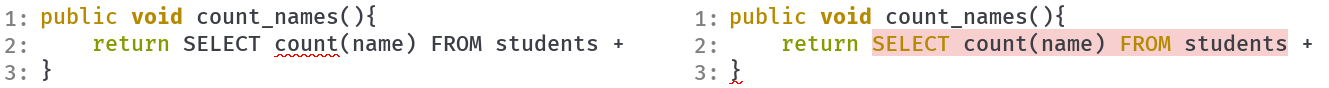
\includegraphics[width=0.90\textwidth]{images/autoboxerrorafterinsert_javasql.png}
\end{center}
\begin{picture}(0,0)
    \put(-242,35.5){\textcolor{black}{\textbf{(a)}}}
    \put(-5,35.5){\textcolor{black}{\textbf{(b)}}}
\end{picture}
\vspace{-1.2em}
\caption{An example showing why parsing too far beyond a candidate language box increases
  the chances of rejecting it. In \textbf{(a)}, we have altered Eco to only insert
candidate language boxes that do not cause subsequent parse errors. However,
the `\texttt{+}` operator is invalid in an SQL \texttt{FROM} clause meaning
that it will be left to the outer language (Java) where it also causes a syntax
error. Thus the candidate language box around the SQL is rejected. In
\textbf{(b)}, we use the heuristic described in Section~\ref{sec:filtering},
where we only filter out candidate language boxes that cause syntax errors in
the first non-whitespace token. Thus although there is still a syntax error in
the program (at the `\texttt{\}}' character), since `\texttt{+}' is valid after
the candidate SQL language box, that candidate is not filtered out.}
\label{fig:autoboxerrorafterinsert}
\end{figure*}

Our filtering heuristic is thus simple: we accept all candidate language
boxes which do not lead to a syntax error at the next non-whitespace token. In other
words, if a language box is syntactically valid at its immediate surrounding
context in the parse tree, we don't mind if it causes errors beyond that
context, since we assume those are the result of an
incomplete program. Note that, by definition, the tokens before the candidate
language box will be valid, so we only need to check those tokens after the
candidate. The reason that we specify that the first non-whitespace
token must not contain an error is that grammars for incremental parsing almost
always define whitespace as a token. This means that the incremental parser
often inserts a whitespace token after a candidate language box, and that
whitespace token is by definition syntactically valid, though not particularly
insightful. We thus need to skip such tokens in order to get to a
token which tells us something useful about the context surrounding a candidate
language box (see Figure~\ref{fig:autobox_nonwhitespace} for an example).
Note that we do not need to check the tokens preceding a candidate language box
for correctness since, by definition, the parser will be in a correct state
at that point.

Similar to the candidates heuristic, the filtering heuristic also uses a
recogniser to confirm candidates, since language boxes need to be virtually
inserted and parsing continued without actually altering the parse tree. Before
we can virtually insert and parse the language box, however, we need to put the
recogniser into the appropriate state. When using the stack heuristic, this
means simply copying the current parsing stack up to the candidate's location.
The other two heuristics require some more preparation, since the chosen
location likely doesn't exist on the current parsing stack. Luckily, there is
no need to reparse the entire program up to the location we want to insert the
language box at. Instead, we can use incremental parsing to skip all subtrees
that are not a direct ancestor of the node after which we want to insert the
language box. This way we can recreate the parsing stack as if we had inserted
the language box at that point and reparsed the changed parse tree (see Figure
\ref{fig_preparse}).


\subsection{Applying or presenting candidates}
\label{applying and presenting}

Once the filtering heuristic has run, we will have zero or more possible
language boxes to insert. If there are zero candidates, then the algorithm
completes. If there is one candidate, we simply insert it to the user's
program. If the user is unhappy with the insertion, they can remove it by
pressing undo (conventionally \keys{Ctrl+Z}). Implemented naively, this isn't
enough, as on each subsequent key press the algorithm may try to insert the
same unwanted language box. Therefore removing a language box in this way marks
a flag \texttt{noinsert} on the node with a syntax error identified by the
consideration heuristic. When set to \texttt{true}, the candidates heuristic
will notice and deliberately ignore such nodes so that language boxes are not
repeatedly inserted.

\begin{figure*}
\begin{center}
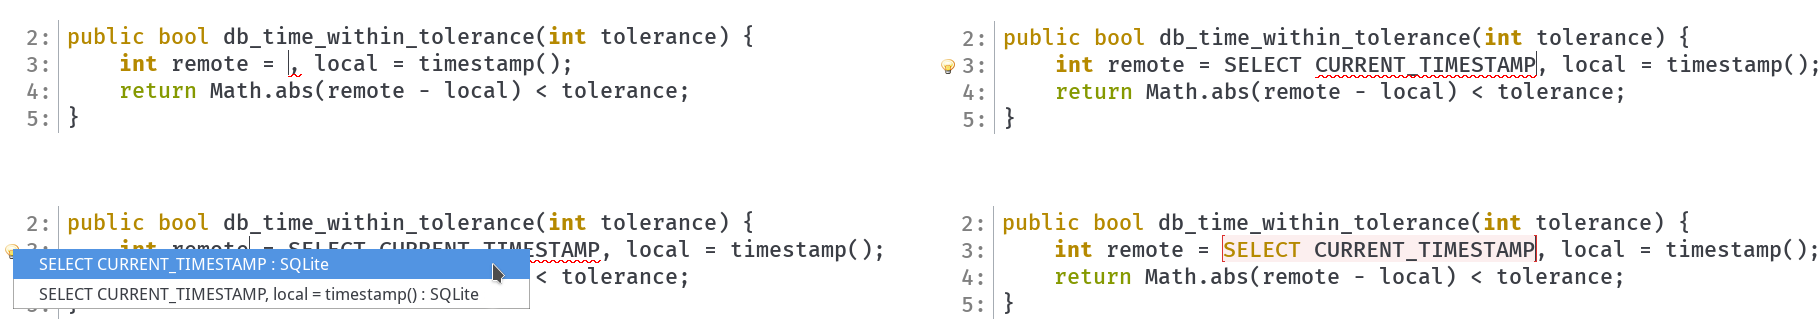
\includegraphics[width=1\textwidth]{images/autobox_multioption_java_sql.png}
\end{center}
\begin{picture}(0,0)
    \put(-255,95){\textcolor{black}{\textbf{(a)}}}
    \put(0,95){\textcolor{black}{\textbf{(b)}}}
    \put(-255,53){\textcolor{black}{\textbf{(c)}}}
    \put(0,53){\textcolor{black}{\textbf{(d)}}}
\end{picture}
\vspace{-1.5em}
\caption{An example of multiple language box candidates in our running Java and SQL
  composition. \textbf{(a)} The user is editing an existing Java programme,
  and has just deleted the expression after \qtt{remote}.
  \textbf{(b)} Inserting an SQL statement leads a syntax error in Java. The
  automatic language box algorithm then finds multiple valid language box
  candidates. Rather than picking one at random, the syntax error remains, and
  the existence of multiple candidates is indicated to the user by the light
  bulb image.
  \textbf{(c)} Clicking on the light bulb displays the candidate language boxes
  that could be inserted. In this example, the user clicks on the first in the
  drop-down list. \textbf{(d)} The appropriate language box is inserted.}
\label{fig:multiplecnds}
\end{figure*}

\label{multiple candidates}
However, if there are multiple candidates, then we have two choices: we could
insert one of the candidates and present the others to the users as choices; or
simply present all the candidates as choices without inserting
any of them. The former approach is surprisingly hard to do well. If we were to
non-deterministically select one candidate and insert it, the user would be
unable to predict what was about to happen on each key press. We could instead
rank candidates (perhaps by `relevance', or length, or starting position etc.),
but we were unable to find a ranking system which matches the user's intentions
often enough to be worthwhile. We therefore simply present all the candidates
as options to the user from which they must choose one (see Figure~\ref{fig:multiplecnds}). As we shall see in
Section~\ref{sec:evaulation}, this happens rarely enough that it is not a
significant problem. It is also worth noting that this is an
example of a fundamental difference between traditional batch parsing and
incremental parsing: it is entirely feasible for us
to ask the user for their help in choosing language boxes as that choice can
be made once and recorded permanently, rather than having to be made anew
on each (batch) parse.


\begin{center}
\end{center}


\subsection{Removing and resizing}

Automatically inserted language boxes start life in the \emph{uncommitted}
state, which means that they can then be considered possible candidates for
automatic removing and resizing. Language boxes move to the \emph{committed}
state when the user shows that they are finished
editing at the current point by moving the cursor outside of the language box.
Users can manually change a committed box to uncommitted if they
later want it to be subject to the algorithm again. If the content of an
uncommitted language box, or its surrounding area, changes then it may be
automatically removed or resized by the algorithm.


\subsubsection{Removing language boxes}

The simplest example of when we might want an automatic language box removed is if
the user deletes a character immediately after an automatic language box has
been inserted. For example, if an SQL language box is inserted as soon as the
user types `\texttt{int x = SELECT * FROM t}` and the user then presses
backspace, the automatic language box should disappear because `\texttt{SELECT
* FROM}' is valid Java and we want to prioritise the outer language in a
composition. As Figure~\ref{fig_autoremoval}) shows, there are other scenarios
when uncommitted language boxes should be removed, including situations where
it is sensible for them to be inserted and removed more than once as the user
types. The complete set of situations we handle are as follows:

\begin{enumerate}
  \item If an uncommitted language box's content causes a syntax error within
    the language box, then the language box should be removed if its contents
    can be successfully parsed in the outer language.
  \item If an uncommitted language box causes a syntax error in the outer
    language then it should be removed if its contents are valid in the
    outer language.
  \item If an uncommitted language box's content is valid in both the inner and
    outer languages, then the language box should be removed if that would not
    then cause subsequent parse errors. Following the precedent from
    Section~\ref{sec:filtering}, we use the first non-whitespace token after
    the language box as a proxy for this.
\end{enumerate}

Not, that while the first two situations are triggered by an error occuring either inside
the box or on the box itself, the third situation has no clear trigger. On each
run of the incremental parser we thus check the third situation for each uncommitted
language box in the program. Fortunately, unless the user has manually marked some
language boxes as uncommitted, the only uncommitted language boxes can be at
the local location, so their number is typically small and the performance
implications trivial.

\begin{figure}
\begin{center}
\vspace{0.8em}
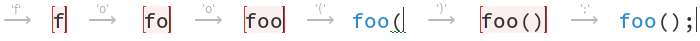
\includegraphics[width=0.45\textwidth]{images/autoremove_foo.png}
\vspace{-0.8em}
\end{center}
\caption{An example showing the constraints for automatic language box removal in practice.
The example uses a composition of PHP and Python where Python expressions are valid at
PHP's top-level.
We can see that as the user types, language boxes are getting automatically
inserted and removed depending on their content. At the beginning the user types
\qtt{f}, which is not valid in PHP and thus gets replaced by a Python
language box, making the program valid again. The box stays until the user
inserts \qtt{(} which makes the Python language box invalid, and since all of
its content can be parsed in the outer language, the box is removed.
As soon as the user inserts the closing bracket \qtt{)}, a Python box is
inserted again to fix the PHP parsing error caused by a missing semicolon. When the
user eventually inserts the missing semicolon the contents of the language box
are valid in both PHP and Python. However, since the box can be removed
without introducing an error, we prioritise the outer
language, and remove it again.}
\label{fig_autoremoval}
\end{figure}


\subsubsection{Resizing language boxes}

Although we do not change the starting position of uncommitted language boxes
(which can be highly distracting), their right hand extent can be automatically
changed to encompass more or less content (Figure~\ref{intro_example} shows an
example of the former). A language boxes is expanded to encompass more content
if: its parse tree does not contain a syntax error; if encompassing the
additional content does not cause a syntax error within the language box; and
if removing the content from the outer language does not cause syntax errors in
the first non-whitespace token in the outer language.
Language boxes are shrunk to encompass less content if they
contain a syntax error and moving the content to the outer language both
fixes the error inside the language box and does not
introduce additional syntax errors in the outer language.

Fortunately both growing and shrinking can be handled with our existing
candidates recogniser (see Section~\ref{sec:recognisers}). When there is a
change \laurie{near/after?}\lukas{this is tricky to define,
since its unclear how far/close an edit needs to happen to affect the box.
currently we only check for shrinking if the box contains errors, while
expansion is checked everytime an edit happens anywhere in the program}\laurie{we have to define it ;) do we check every uncommitted language box on every parse or ...?} or inside
an uncommitted language
box, we run our altered candidates recogniser at the start of the language box.
This returns all the possible right hand extents of the language box. Starting
from the candidate which matches the most content and working backwards, we then
filter out candidates which do not meet the above conditions. If none remain,
the algorithm completes; if one remains,
we resize the language box appropriately; if more than one remains, we present
the multiple options to the user in the same way as in Section~\ref{multiple candidates}.


\subsection{Highly ambiguous compositions}
\label{sec:highly ambiguous compositions}

Some language compositions are so fundamentally ambiguous that normal automatic
language boxes do not work well. For example, consider a composition of Java
(or any other programming language!) with HTML, where HTML language boxes can
be used wherever Java expressions are valid. Since HTML's lexer can match
almost any text, nearly all errors in Java can be resolved by wrapping text in
an HTML language box, which is unlikely to match the user's intentions.

To solve many such cases, we thus have to relax the `no hints' constraint from
Section~\ref{the problem} by allowing language composition authors to specify
either of both of: those \laurie{token types or strings?} which can start a
language box; and those which can't start a language box. For example, in the
case of the Java and HTML composition, a good choice for the language
composition is to specify HTML tags as being the only valid starting input for
a candidate language box. \laurie{i assume we enforce this in the candidates
recogniser so that later stages don't have to do needless work?}


\section{Limitations}
\label{sec:lbox_limitations}

Simplifying somewhat, automatic language boxes can be seen as implementing a
simplified, predictable, online variant of generalised parsing. Since they are
simplified there are situations where they do not perform as well as hoped.
Although (as we shall see in Section~\ref{sec:evaluation}) these cases are
rare, it is useful to enumerate some of their fundamental weaknesses.

Although our solution to highly ambiguous compositions (see Section~\ref{highly
ambiguous compositions}) works well when the outer language matches specific
input (e.g.~Java) and the inner language matches nearly anything (e.g.~HTML),
the reverse does not work well. For example, if we compose HTML and Java where
Java expressions are valid wherever HTML tags are valid, automatic language
boxes almost never trigger, since there are few ways of making a syntax error
in HTML. We are unable to imagine a solution to this problem.

\subsection{Wrong detection}

Sometimes, while the user is typing, language boxes are inserted prematurely,
and wrap contents of the outer language into the language box, that weren't
meant to be part of it.
For example, this can occur when composing Java and Python,
allowing Java functions to be replaced with Python functions, as shown below:

\begin{center}
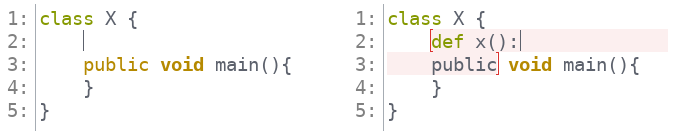
\includegraphics[width=0.50\textwidth]{images/autobox_limitjavapy.png}
\end{center}

The user attempted to insert a Python function above the Java function.
However, as the user was typing, a box was automatically inserted which
extended into the Java function, and used the keyword \qtt{public} as the body
of the Python function.  This is valid, since the keyword is optional in Java,
so the insertion of that box does not create any errors, even though it is
clearly not what the user intended.

Though this is alleviated in many cases by shrinking the box again once more
information has become available, it remains a problem in some compositions.
To circumvent this problem, we added a flag which restricts the recogniser
to consume text that was created before the contents of the putative language
box. This is made possible by using the history of the parse tree, e.g.~we simply
need to check if a consumed tokens version number is smaller than the first token
in the language box, and if that is the case, it is rejected, and the recogniser
stops.
The idea behind this is based on the assumption that the user is likely to type
language box insertions consecutively, which works well on the above example:
since the \qtt{public} token was
typed before the user started typing the Python code, it won't be included in
the box, thus avoiding this issue. The downside to this is, however, that it won't be possible for
the user to type language boxes out-of-order.  For example, they can't start
typing the body of a Python function and add the method header afterwards, as
then the body will be older than the header.

\subsection{Grammar limitations}

\lukas{this is partially solved by the line heuristic, unless we insert a newline
into the examples below.}

Sometimes the structure of a grammar can be responsible for the failure to
generate automatic language boxes. For example, let's consider a composition of
PHP and Python, that allows Python expressions wherever PHP expressions are
valid. The user then edits the composition as follows:

\begin{center}
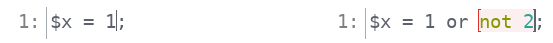
\includegraphics[width=0.45\textwidth]{images/autobox_limitphpgrammar.png}
\end{center}

The user might reasonably expect to have a second option here, which would
allow the content \qtt{1 or not 2} to be wrapped into a Python language box.
The algorithm, however, couldn't detect this and instead only found a single
candidate, \qtt{not 2}, which was automatically inserted.  The problem lies
within the PHP grammar, which also has a keyword \qtt{or}, and how the location
for language box candidates are calculated. As described earlier in this
chapter, we use a technique similar to error recovery, that rewinds the parse
stack to find a position on the stack, where the language can be inserted.
However, the way the PHP grammar is structured and thus parses the above input,
makes it impossible to find a location on the stack that allows \qtt{1 or not
2} to be wrapped into a language box, as Figure \ref{fig_auto_phplimit} shows.

\begin{figure}
\begin{center}
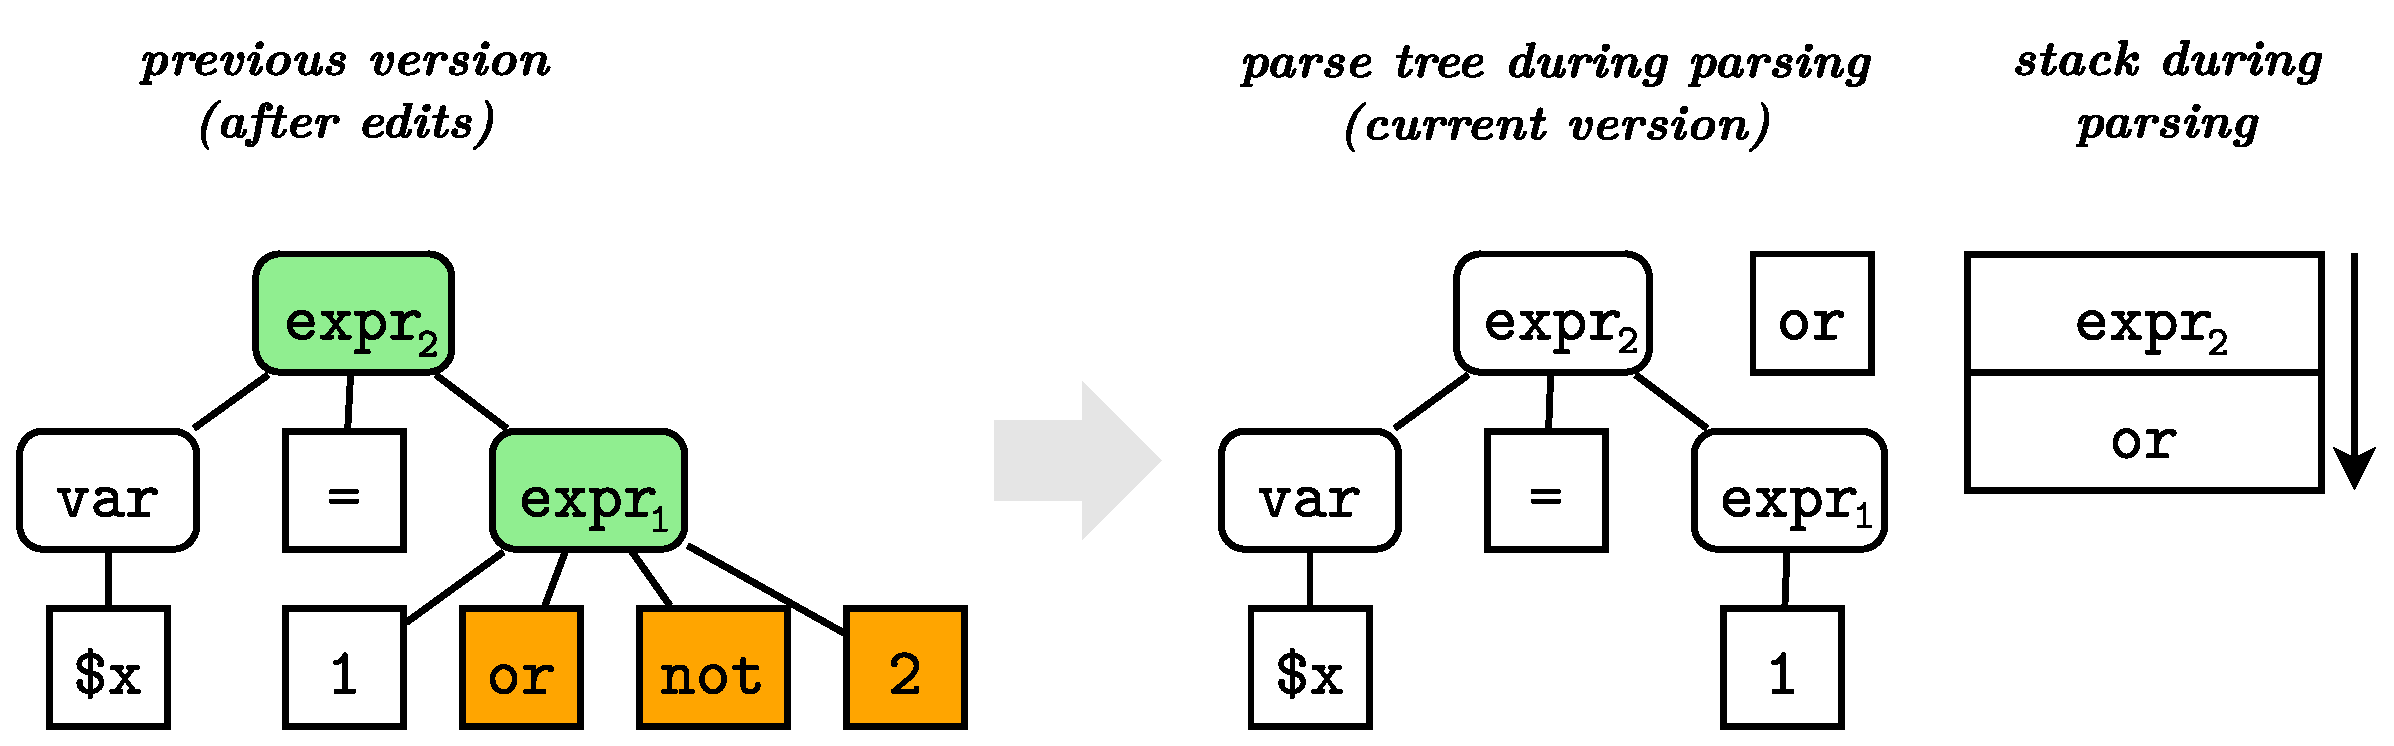
\includegraphics[width=0.49\textwidth]{images/limitation_php}
\end{center}
\caption{An example showing how sometimes the grammar of a language can
keep the automatic language box detection from finding appropriate candidates.
Shown on the left is the elided parse tree after the user edited the PHP expression
\qtt{\$x = 1;} by inserting the Python code \qtt{or not 2}. However, we
can see on the right, that by the time the error occurs, PHP has already reduced \qtt{\$x = 1} to \texttt{expr\textsubscript{2}}, and shifted
\texttt{or} onto the stack. The only valid locations for a language
box we can thus find are before \texttt{expr\textsubscript{2}} and \qtt{or}. In particular,
we cannot find the location before \qtt{1} which would allow us to wrap the entire expression
into a box.}
\label{fig_auto_phplimit}
\end{figure}

Other compositions suffer from the same issue:
\begin{itemize}
    \item[JavaLua] `\verb|int x = 1, 2|', can't wrap `\verb|1, 2|' in a Lua
        language box, since Java has already reduced parts of the parse tree
        after seeing the `\texttt{,}', so that neither heuristic can reach the
        beginning of the expression.
    \item[JavaSQL] `\verb|int x = BEGIN; SELECT a FROM t;|'. Since `\texttt{BEGIN;}` is a
        valid Java expression, it has already been reduced to a subtree which
        can't be reached from the error that occurs in `\texttt{FROM}'.
    \item[LuaJava] `\verb|x = new int[1]|'. Error occurs after the Java expr, at
        which point it has already been reduced in Lua.
    \item[LuaSQL] `\verb|local x = SELECT a, b FROM t1;|'. After parsing
        `\texttt{,}', the parse tree is reduced in a way that makes reaching the
        beginning of the expression impossible for the heuristics.
    \item[LuaSQL] `\verb|local x = SELECT a.b FROM t1;]|'. Same as the above but
        with `\texttt{.}' instead of `\texttt{,}'.
\end{itemize}

\subsection{Problems with comments}

Sometimes comments can be the reason for a failed insertion. For example, when
composing Lua and Java, a possible composed program may look like this:

\begin{lstdefault}[language={[5.2]Lua}]
function decrease(x)
    y = --x
    return y
end
\end{lstdefault}

where `\verb|--x|' is meant to be a Java expression. However, since `\texttt{--}'
in Lua is a comment, the error happens later in `\texttt{return}', making it
impossible for the heuristic to find the beginning of the expression.
Similarly, when composing Java and Lua while using Lua's floor division, e.g.~
`\verb|int x = 3//4 + 1;|', no language box is inserted, as `\texttt{//}' is interpreted
as a Java comment, which means the error occurs at a location which makes it impossible
for the heuristic to find the beginning of the expression.

Another problem with comments appears in compositions of PHP and SQL:

\begin{lstdefault}[language=PHP]
$x = SELECT a FROM t1 -- comment;
$y = 2;
\end{lstdefault}

At first, when typing the SQL statement, as language box is correctly inserted
around \verb|SELECT a FROM t1|. However, after typing the first \texttt{-}
inside the language box, the box is shrunken, moving the \texttt{-} to the
outside. One would assume that the box gets expanded again as soon as we
continue typing the comment. However, when testing if the box can be expanded,
the lexer for SQLite lexes the entire comment to the end of the line, including
the semicolon finishing the PHP statement. Without this semicolon, PHP cannot
parse successfully, breaking the condition for the expansion, which is thus
aborted. The same problem can appear in other compositions where semicolons are
used to end a statement, e.g.~Java.

\subsection{Problems with strings}

Some languages, like PHP, allow newlines within strings. Embedding such a
language inside another language can thus sometimes require the entire file to
be lexed during automatic language box detection. For example when typing the
PHP expression \texttt{\$x = 'a'} into Java, this will cause the entire
remaining Java program to be lexed as long as the single quote has not been
closed. However, since the lexing only happens virtually and is not applied to
the input (unless this result in the insertion of a new language box), this
does not affect the parse tree of the outer language. And since lexing is
generally quite fast, the performance impact will also be insignificant.


\section{Orphan}

\subsection{Incremental Recogniser for auto removal}
\label{sec:impl_removerec}

Section \ref{subsec_autoremoval} described how automatically inserted language
boxes can automatically be removed again, if they become invalid. The condition
for this is that the box's content is valid in the outer language.  In essence,
we need to temporarily remove the language box, paste its content where the box
was before, and then check if the program can still be parsed; of course
without actually altering the parse tree. A recogniser is thus again a good
choice. In order to test if the contents of the box are valid in the outer
language, we first need to initialise the recogniser to the state just before
the language box would be parsed. We can do this incrementally, by only
traversing subtrees that are direct ancestors of the language box. All other
subtrees can be skipped (i.e.~incrementally shifted) similar to the default
incremental parser.

This process is implemented via an additional method \texttt{preparse}, which
incrementally initialises a recogniser's parsing state to the state just before
a given node. Figure \ref{fig_preparse} shows an example of a parse tree, where
we want to test if a language box can be removed, and the algorithm to
initialise the recogniser.
After the recogniser has been initialised, we simply use \texttt{consume\_text}
to parse the content of the language box. If the entirety of the language box
can be successfully parsed in the outer language, the box can be removed.  Of
course, depending on the parsing status of the box, we may also need to parse
at least one non-whitespace token following the former language box.

\begin{figure}
\begin{minipage}{0.45\textwidth}
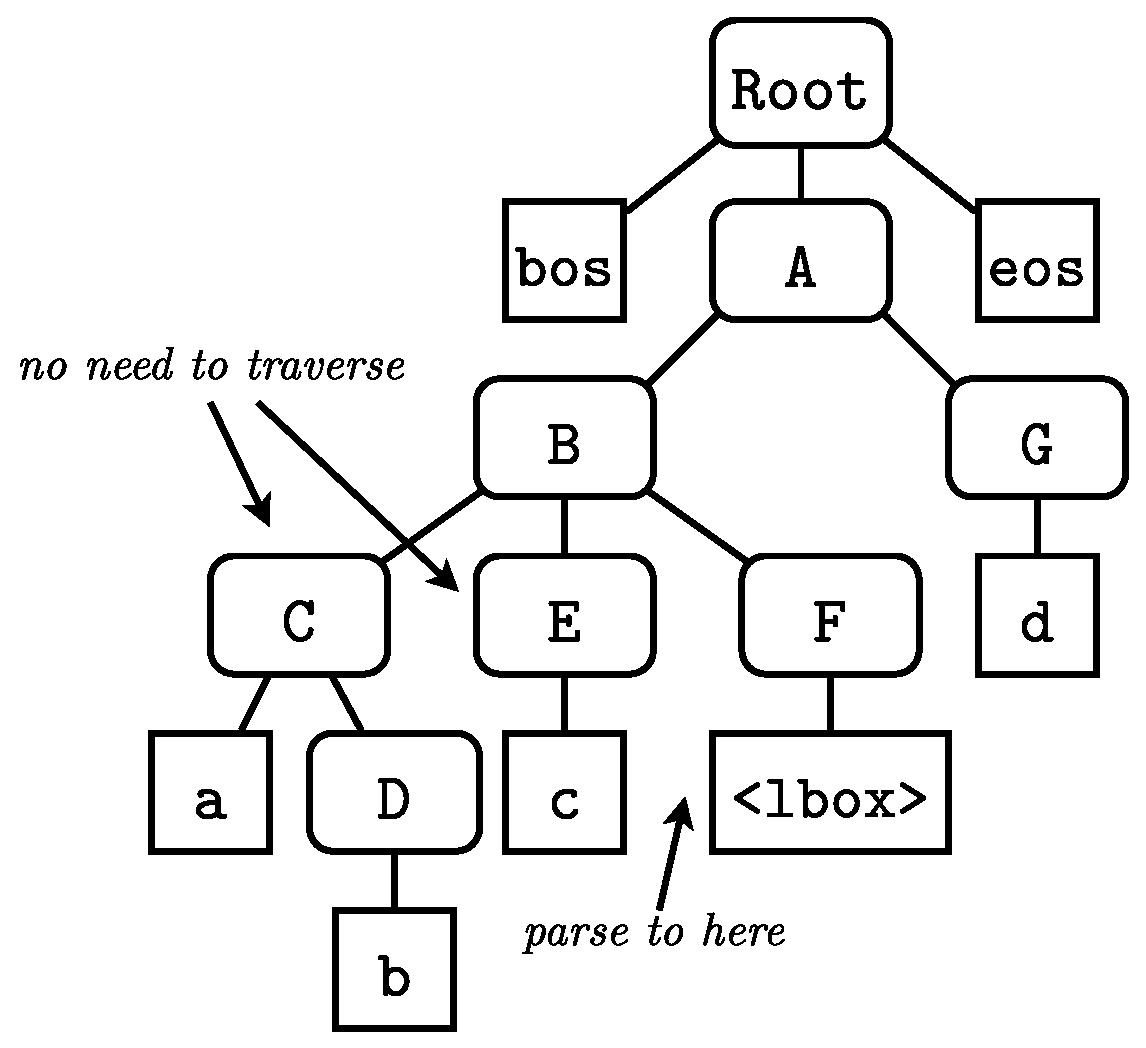
\includegraphics[width=0.9\textwidth]{images/autoremoval}
\end{minipage}
\begin{minipage}{0.5\textwidth}
\begin{lstdefault}[basicstyle=\linespread{1.0}\footnotesize\ttfamily]
def preparse(bos, lbox, parser):
  # "mark" ancestors of lbox
  path_to_lbox = set()
  parent = lbox.parent
  while parent is not <!\textit{Root}!>:
    path_to_lbox.add(parent)
    parent = parent.parent

  # initialise parser
  node = bos
  while node is not lbox:
    if node not in path_to_lbox:
      parser.parse(node)
    else: # traverse node
      if node.children:
        node = node.children[0]
      else:
        node = node.right_neighbour()
\end{lstdefault}
\end{minipage}
\caption{A parse tree with a language box that we want to automatically remove (left)
and the preparse-algorithm (right). In
order to test if the box's content is valid in the outer language, we
initialise a recogniser to the state just before we would parse the language box,
using the recogniser's \texttt{preparse} method. This is done,
by `marking' the ancestors of the language box, as if the language box
contained changes (lines 3--7), and then incrementally parse those subtrees
up to the box (lines 10--18).}
\label{fig_preparse}
\end{figure}


\section{Evaluation}
\label{sec:evaluation}

To evaluate the accuracy of automatic language boxes, we ran an experiment,
testing each heuristic on multiple benchmarks. Each benchmark uses a
compositions of two languages, where expressions or functions from one language
can be embedded into the other. The benchmark then first chooses a random file
that parses in the main language. It then picks a random expressions or
function written in the embedded language, and inserts it at a valid location
in the chosen file. All files and expressions/functions were extracted from
real-world programs.

Figure \ref{tbl_valid} shows the total percentage of
acceptable outcomes for each heuristic used broken down by each composition.
Acceptable outcomes are one of the following: a language box gets succesfully
inserted; no language box was inserted since the insertion was already valid in
the outer language; the insertion had multiple options which are presented to
the user.

The results show that while each heuristic has weaknesses, when put together
they result in over 96\% of acceptable outcomes. Weaknesses in the heuristics
are based on the composition. For example, the history-based heuristic only
achieves 67\% of acceptable outcomes when used on the Java+Lua composition. The
reason for this low number can be accounted to the insertion of Lua functions
right after a Java comment.  Since the insertion is attached to the comment
subtree, the history-based heuristic is not able to find a valid location for
the language box by traversing the parse tree.  The line-based heuristic on the
other hand has difficulties with the composition of Java+PHP. The reason for
this is that PHP's function syntax is similar to Java's, e.g.~\texttt{function
x() \{\}} is a valid Java function, where \texttt{function} represents a type.
This leads to many errors only occuring in one of the following lines, which
the line-based heuristic can not deal with. The stack-based heuristic also has
a weakness with the composition of Lua+SQLite. The problem here is related to
the way Lua parses certain inputs. For example, when composing \texttt{x =
SELECT a, b FROM t}, everything up to `\texttt{b}' can be parsed in Lua,
leading to a reduction. This reduction removes \texttt{SELECT} from the stack,
replacing it with a subtree and making it impossible to find a valid location
to insert a language box at.

\begin{figure*}[hbt]
    \begin{tabular}{l  c  c  c  c  c  c  c  c  c  c  c  c  c }
    \toprule
        & \rotatebox{65}{JavaLua} & \rotatebox{65}{JavaPHP} & \rotatebox{65}{JavaSQLite} & \rotatebox{65}{LuaJava} & \rotatebox{65}{LuaPHP} & \rotatebox{65}{LuaSQLite} & \rotatebox{65}{PHPJava} & \rotatebox{65}{PHPLua} & \rotatebox{65}{PHPSQLite} & \rotatebox{65}{SQLiteJava} & \rotatebox{65}{SQLiteLua} & \rotatebox{65}{SQLitePHP} & \rotatebox{65}{Overall} \\
    \midrule
    Corpus size & 950 & 889 & 659 & 295 & 265 & 170 & 557 & 500 & 317 & 282 & 289 & 281 & 5,454 \\
    \midrule
    All & 99.4\% & 94.6\% & 99.7\% & 97.9\% & 95.9\% & 97.6\% & 99.2\% & 99.2\% & 100.0\% & 97.9\% & 95.2\% & 94.3\% & 97.6\% \\
    Parse tree & 67.4\% & 90.7\% & 99.5\% & 97.5\% & 86.2\% & 90.0\% & 95.9\% & 53.1\% & 100.0\% & 96.8\% & 99.0\% & 96.8\% & 89.4\% \\
    Stack & 97.6\% & 94.5\% & 99.5\% & 96.2\% & 94.3\% & 69.4\% & 99.2\% & 98.1\% & 100.0\% & 97.5\% & 95.2\% & 94.0\% & 94.6\% \\
    Line & 97.5\% & 79.3\% & 99.2\% & 98.2\% & 96.2\% & 96.5\% & 99.2\% & 98.2\% & 99.7\% & 97.9\% & 99.3\% & 96.1\% & 96.4\% \\
    \bottomrule
\end{tabular}
        

    \caption{The total percentage of acceptable outcomes for each benchmark and
    heuristic. Acceptable outcomes are one of the following: a language box
    gets succesfully inserted; no language box was inserted since the insertion
    was already valid in the outer language; the insertion had multiple options
    which are presented to the user. In other words, the total percentage
    doesn't include invalid insertions of language boxes and errors for which
    no language box could be found automatically.}
    \label{tbl_valid}
\end{figure*}

\begin{figure*}[hbt]
    \begin{tabular}{l  c  c  c  c  c  c  c }
    \toprule
        & \multicolumn{1}{p{2cm}}{\centering Complete insertion\\(No errors)} & \multicolumn{1}{p{2cm}}{\centering Partial insertion\\(No errors)} & \multicolumn{1}{p{2cm}}{\centering Partial insertion\\(Errors)} & \multicolumn{1}{p{2cm}}{\centering No insertion\\(Valid)} & \multicolumn{1}{p{2cm}}{\centering No insertion\\(Errors)} & \multicolumn{1}{p{2cm}}{\centering No insertion\\(Multi)} \\
    \midrule
    All & 66.1\% & 2.6\% & 2.4\% & 24.9\% & 0.7\% & 3.2\% \\
    Parse tree & 59.6\% & 2.5\% & 1.2\% & 25.0\% & 9.9\% & 1.7\% \\
    Stack & 65.5\% & 2.6\% & 2.4\% & 24.9\% & 2.5\% & 2.0\% \\
    Line & 65.4\% & 2.4\% & 2.1\% & 25.0\% & 2.8\% & 2.3\% \\
    \bottomrule
\end{tabular}
        

    \caption{Overall performance of the different
    heuristics on all benchmarks per outcome category. The categories are:
    \textbf{Valid insertion}, a language box was successfully inserted, \textbf{Invalid insertion},
    a language box was inserted but it did not fix the error or introduced new
    ones, \textbf{No insertion (Valid)}, no language box was inserted because the inserted
    code fragment is valid syntax, \textbf{No insertion (Error)}, no language box could be
    found to fix the error, \textbf{No insertion (Multi)}, multiple language box options
    were found.}
    \label{tbl_breakdown}
\end{figure*}


\section{Related Work}
\label{autobox_related_work}

Scannerless parsing~\cite{visser97scannerless, vandenbrand02disambiguation} is well
suited for language composition since it can parse any context-free grammars
which are closed under composition. A notable example of this is
Spoofax~\cite{kats10spoofax}, a language workbench for extending and composing
context-free grammars.
Although scannerless parsing can parse ambiguous programs by creating a parse
forest, it is still necessary to reduce the parse forest into a single
parse tree in order to compile or interpret it. A common way to reduce the parse forest is to
remove all parse trees that are invalid when considering additional information
about the input, such as types~\cite{vinju05typedriven}. Using type information can avoid the
need for separators to disambiguate languages in many cases, however still
requires a set of disambiguation rules, such as preferring identifiers in the
outer language (i.e.~the meta language) over those in the inner language
(i.e.~the object language), or choosing the shortest path if multiple valid
options are available. Unfortunately, not all ambiguities can be solved this
way, making the use of separators still a necessity.

Choosing separators is not trivial, since they can still introduce ambiguities
if the same separator symbol is used for different nonterminals of the embedded
language. This requires \textit{explicit disambiguation}, i.e.~using a
different separator for each embedding with a different nonterminal symbol,
e.g.~\verb|cls{...}cls| for embedding classes and \verb|func{...}func| for
functions~\cite{batory98jts}. Since this can
quickly cause ``syntactic clutter``~\cite[p.~4]{bravenboer05generalized},
an alternative solution is to use type information to automatically disambiguate
embeddings, thus reducing the amount of unique separators that would otherwise
be required~\cite{zook04generating, bravenboer05generalized}.
Unfortunately, since these approaches are dependent on types, they do not work
for dynamically typed languages. Furthermore, heuristics such as picking the
shortest path on multiple valid options can hide options the user cares about
(as shown in Section~\ref{auto_handling_multiple_solutions}).

Despite these improvements, Spoofax's grammar definition SDF,
which allows arbitrary CFGs, can give no guarantees that its grammars are unambiguous,
even more so when they are composed together, since composing two unambiguous grammars can lead to an ambiguous one.
Spoofax thus uses reject grammars, which solve this problem, but
make such grammars context-sensitive~\cite{eijck__lets_accept_rejects}.

Another notable example for language composition is Copper~\cite{wyk07context}
which implements a context-aware scanner to solve ambiguities in language
compositions. The basic idea is that the parser can tell the scanner which
tokens it can parse next and the scanner can only return results from that list.
This means that if two composed languages have similar tokens (e.g.~keywords,
identifiers), the lexer solves ambiguities
by returning the token for the language that it is currently parsing (i.e.~that is currently in context). This allows
Copper to compose languages by extending the host language's grammar rules
with references to rules in the embedded language. However, at the point where
another language can be embedded, i.e.~where the two languages meet, a token
may be valid in both the host as well as the embedded language.
Copper solves this problem
via \texttt{dominates} clauses which are defined within the lexing rules. For example, if an
identifier in the host language clashes with a keyword in the embedded language,
then we can define a clause that says that the keyword dominates the identifier
and needs to be prioritised. Unfortunately, this has the
downside that those tokens cannot be used in the host language at that point,
restricting the host language's expressiveness. This also means that each
composition needs to determine all of those cases and modify grammar and lexer in ways that solve
these ambiguities, making it impossible to create a one-size-fits-all solution for
arbitrary compositions.


\bibliography{bib}

\appendix

\section{Tables}
\subsection{Breakdown: All heuristics}
\begin{tabular}{l  c  c  c  c  c  c  c }
    \toprule
        & \multicolumn{1}{p{2cm}}{\centering Complete insertion\\(No errors)} & \multicolumn{1}{p{2cm}}{\centering Partial insertion\\(No errors)} & \multicolumn{1}{p{2cm}}{\centering Partial insertion\\(Errors)} & \multicolumn{1}{p{2cm}}{\centering No insertion\\(Valid)} & \multicolumn{1}{p{2cm}}{\centering No insertion\\(Errors)} & \multicolumn{1}{p{2cm}}{\centering No insertion\\(Multi)} \\
    \midrule
    JavaLua & 62.0\% & 1.8\% & 0.3\% & 31.4\% & 0.4\% & 4.1\% \\
    JavaPHP & 84.3\% & 5.2\% & 4.2\% & 2.6\% & 1.7\% & 2.1\% \\
    JavaSQL & 94.1\% & 0.3\% & 0.5\% & 4.9\% & 0.2\% & 0.2\% \\
    LuaJava & 51.6\% & 2.1\% & 2.4\% & 42.4\% & 1.5\% & 0.0\% \\
    LuaPHP & 88.5\% & 5.6\% & 3.3\% & 0.7\% & 2.0\% & 0.0\% \\
    LuaSQL & 90.0\% & 1.6\% & 0.0\% & 5.3\% & 3.2\% & 0.0\% \\
    PHPJava & 38.4\% & 3.4\% & 0.2\% & 49.4\% & 0.2\% & 8.5\% \\
    PHPLua & 51.5\% & 3.1\% & 0.4\% & 38.7\% & 0.0\% & 6.2\% \\
    PHPSQL & 91.9\% & 0.0\% & 2.0\% & 6.2\% & 0.0\% & 0.0\% \\
    SQLJava & 29.4\% & 0.7\% & 2.5\% & 63.5\% & 0.0\% & 3.9\% \\
    SQLLua & 26.3\% & 4.8\% & 5.5\% & 54.3\% & 0.0\% & 9.0\% \\
    SQLPHP & 66.9\% & 0.4\% & 14.2\% & 16.7\% & 0.0\% & 1.8\% \\
    \bottomrule
\end{tabular}
        

\subsection{Breakdown: History-based heuristic}
\begin{tabular}{l  c  c  c  c  c  c  c }
    \toprule
        & \multicolumn{1}{p{2cm}}{\centering Complete insertion\\(No errors)} & \multicolumn{1}{p{2cm}}{\centering Partial insertion\\(No errors)} & \multicolumn{1}{p{2cm}}{\centering Partial insertion\\(Errors)} & \multicolumn{1}{p{2cm}}{\centering No insertion\\(Valid)} & \multicolumn{1}{p{2cm}}{\centering No insertion\\(Error)} & \multicolumn{1}{p{2cm}}{\centering No insertion\\(Multi)} \\
    \midrule
    SQLiteJava & 29.8\% & 0.4\% & 1.4\% & 63.8\% & 1.8\% & 2.8\% \\
    LuaPHP & 78.0\% & 5.6\% & 3.0\% & 0.7\% & 12.8\% & 0.0\% \\
    LuaJava & 51.0\% & 1.8\% & 1.8\% & 42.4\% & 3.0\% & 0.0\% \\
    SQLitePHP & 69.4\% & 0.4\% & 10.7\% & 16.7\% & 1.4\% & 1.4\% \\
    JavaLua & 39.5\% & 0.3\% & 0.0\% & 31.4\% & 26.4\% & 2.4\% \\
    LuaSQLite & 89.5\% & 1.1\% & 0.0\% & 5.3\% & 4.2\% & 0.0\% \\
    PHPLua & 25.6\% & 0.8\% & 0.2\% & 38.7\% & 29.4\% & 5.4\% \\
    JavaPHP & 82.7\% & 4.8\% & 0.6\% & 2.6\% & 9.1\% & 0.0\% \\
    JavaSQLite & 94.8\% & 0.2\% & 0.0\% & 4.9\% & 0.2\% & 0.0\% \\
    SQLiteLua & 32.2\% & 1.4\% & 2.1\% & 55.4\% & 0.3\% & 8.7\% \\
    PHPJava & 38.6\% & 10.1\% & 0.2\% & 49.4\% & 0.2\% & 1.6\% \\
    PHPSQLite & 92.2\% & 0.0\% & 1.6\% & 6.2\% & 0.0\% & 0.0\% \\
    \bottomrule
\end{tabular}
        

\subsection{Breakdown: Stack-based heuristic}
\begin{tabular}{l  c  c  c  c  c  c  c }
    \toprule
        & \multicolumn{1}{p{2cm}}{\centering Complete insertion\\(No errors)} & \multicolumn{1}{p{2cm}}{\centering Partial insertion\\(No errors)} & \multicolumn{1}{p{2cm}}{\centering Partial insertion\\(Errors)} & \multicolumn{1}{p{2cm}}{\centering No insertion\\(Valid)} & \multicolumn{1}{p{2cm}}{\centering No insertion\\(Error)} & \multicolumn{1}{p{2cm}}{\centering No insertion\\(Multi)} \\
    \midrule
    JavaLua & 59.9\% & 2.0\% & 0.1\% & 31.4\% & 2.8\% & 3.8\% \\
    JavaPHP & 85.8\% & 5.3\% & 4.4\% & 2.6\% & 1.7\% & 0.2\% \\
    JavaSQLite & 94.1\% & 0.3\% & 0.5\% & 4.9\% & 0.2\% & 0.2\% \\
    LuaJava & 50.1\% & 2.1\% & 2.4\% & 42.4\% & 3.0\% & 0.0\% \\
    LuaPHP & 86.9\% & 5.6\% & 3.3\% & 0.7\% & 3.6\% & 0.0\% \\
    LuaSQLite & 62.1\% & 0.5\% & 0.0\% & 5.3\% & 32.1\% & 0.0\% \\
    PHPJava & 45.3\% & 3.5\% & 0.2\% & 49.4\% & 0.2\% & 1.4\% \\
    PHPLua & 49.8\% & 3.1\% & 0.6\% & 38.7\% & 2.1\% & 5.6\% \\
    PHPSQLite & 91.9\% & 0.0\% & 2.0\% & 6.2\% & 0.0\% & 0.0\% \\
    SQLiteJava & 29.8\% & 0.7\% & 2.5\% & 63.5\% & 0.0\% & 3.5\% \\
    SQLiteLua & 27.0\% & 5.2\% & 5.5\% & 54.3\% & 0.0\% & 8.0\% \\
    SQLitePHP & 66.9\% & 0.4\% & 14.2\% & 16.7\% & 0.0\% & 1.8\% \\
    \bottomrule
\end{tabular}
        

\subsection{Breakdown: Line-based heuristic}
\begin{tabular}{l  c  c  c  c  c  c  c }
    \toprule
        & \multicolumn{1}{p{2cm}}{\centering Complete insertion\\(No errors)} & \multicolumn{1}{p{2cm}}{\centering Partial insertion\\(No errors)} & \multicolumn{1}{p{2cm}}{\centering Partial insertion\\(Errors)} & \multicolumn{1}{p{2cm}}{\centering No insertion\\(Valid)} & \multicolumn{1}{p{2cm}}{\centering No insertion\\(Error)} & \multicolumn{1}{p{2cm}}{\centering No insertion\\(Multi)} \\
    \midrule
    SQLiteJava & 29.4\% & 0.7\% & 1.8\% & 63.8\% & 0.7\% & 3.5\% \\
    LuaPHP & 88.9\% & 5.6\% & 3.0\% & 0.7\% & 2.0\% & 0.0\% \\
    LuaJava & 51.9\% & 2.1\% & 2.1\% & 42.4\% & 1.5\% & 0.0\% \\
    SQLitePHP & 67.3\% & 0.4\% & 13.9\% & 16.7\% & 0.0\% & 1.8\% \\
    JavaLua & 60.5\% & 1.8\% & 0.3\% & 31.4\% & 1.9\% & 4.1\% \\
    LuaSQLite & 90.0\% & 1.6\% & 0.0\% & 5.3\% & 3.2\% & 0.0\% \\
    PHPLua & 50.8\% & 2.7\% & 0.4\% & 38.7\% & 1.0\% & 6.3\% \\
    JavaPHP & 75.7\% & 4.6\% & 4.2\% & 2.6\% & 12.6\% & 0.3\% \\
    JavaSQLite & 93.8\% & 0.5\% & 0.5\% & 4.9\% & 0.5\% & 0.0\% \\
    SQLiteLua & 30.8\% & 2.1\% & 2.4\% & 55.0\% & 0.0\% & 9.7\% \\
    PHPJava & 45.0\% & 3.7\% & 0.2\% & 49.4\% & 0.2\% & 1.6\% \\
    PHPSQLite & 91.9\% & 0.0\% & 2.0\% & 6.2\% & 0.0\% & 0.0\% \\
    \bottomrule
\end{tabular}
        



\end{document}
